\chapter{Stencil Computation over Structured Meshes and Parallel Programming in Multicore Architectures}
This chapter will be focusing on stencil computation and its development over the recent years due to the complex nature of modern computer architectures involving chip multicore processors (CMP) and heterogeneous system architectures. I will give a thorough description of stencil computation, CMP-systems as well as parallelization of such problems, methods and optimizations on structured meshes

\section{Introduction}
Stencil computations are operations performed by many numerical methods in the context of scientific  applications. A \textit{stencil} is a geometric pattern of a nodal group centered around some point using information from its neighbor elements, as shown in figure \ref{I_Five_point_stencil_illustration.png}. A stencil operation can be done over a mesh using series of time sweeps to update its value using neighboring values at which the stencil is centered.
\begin{figure}[h]
 \centering 
     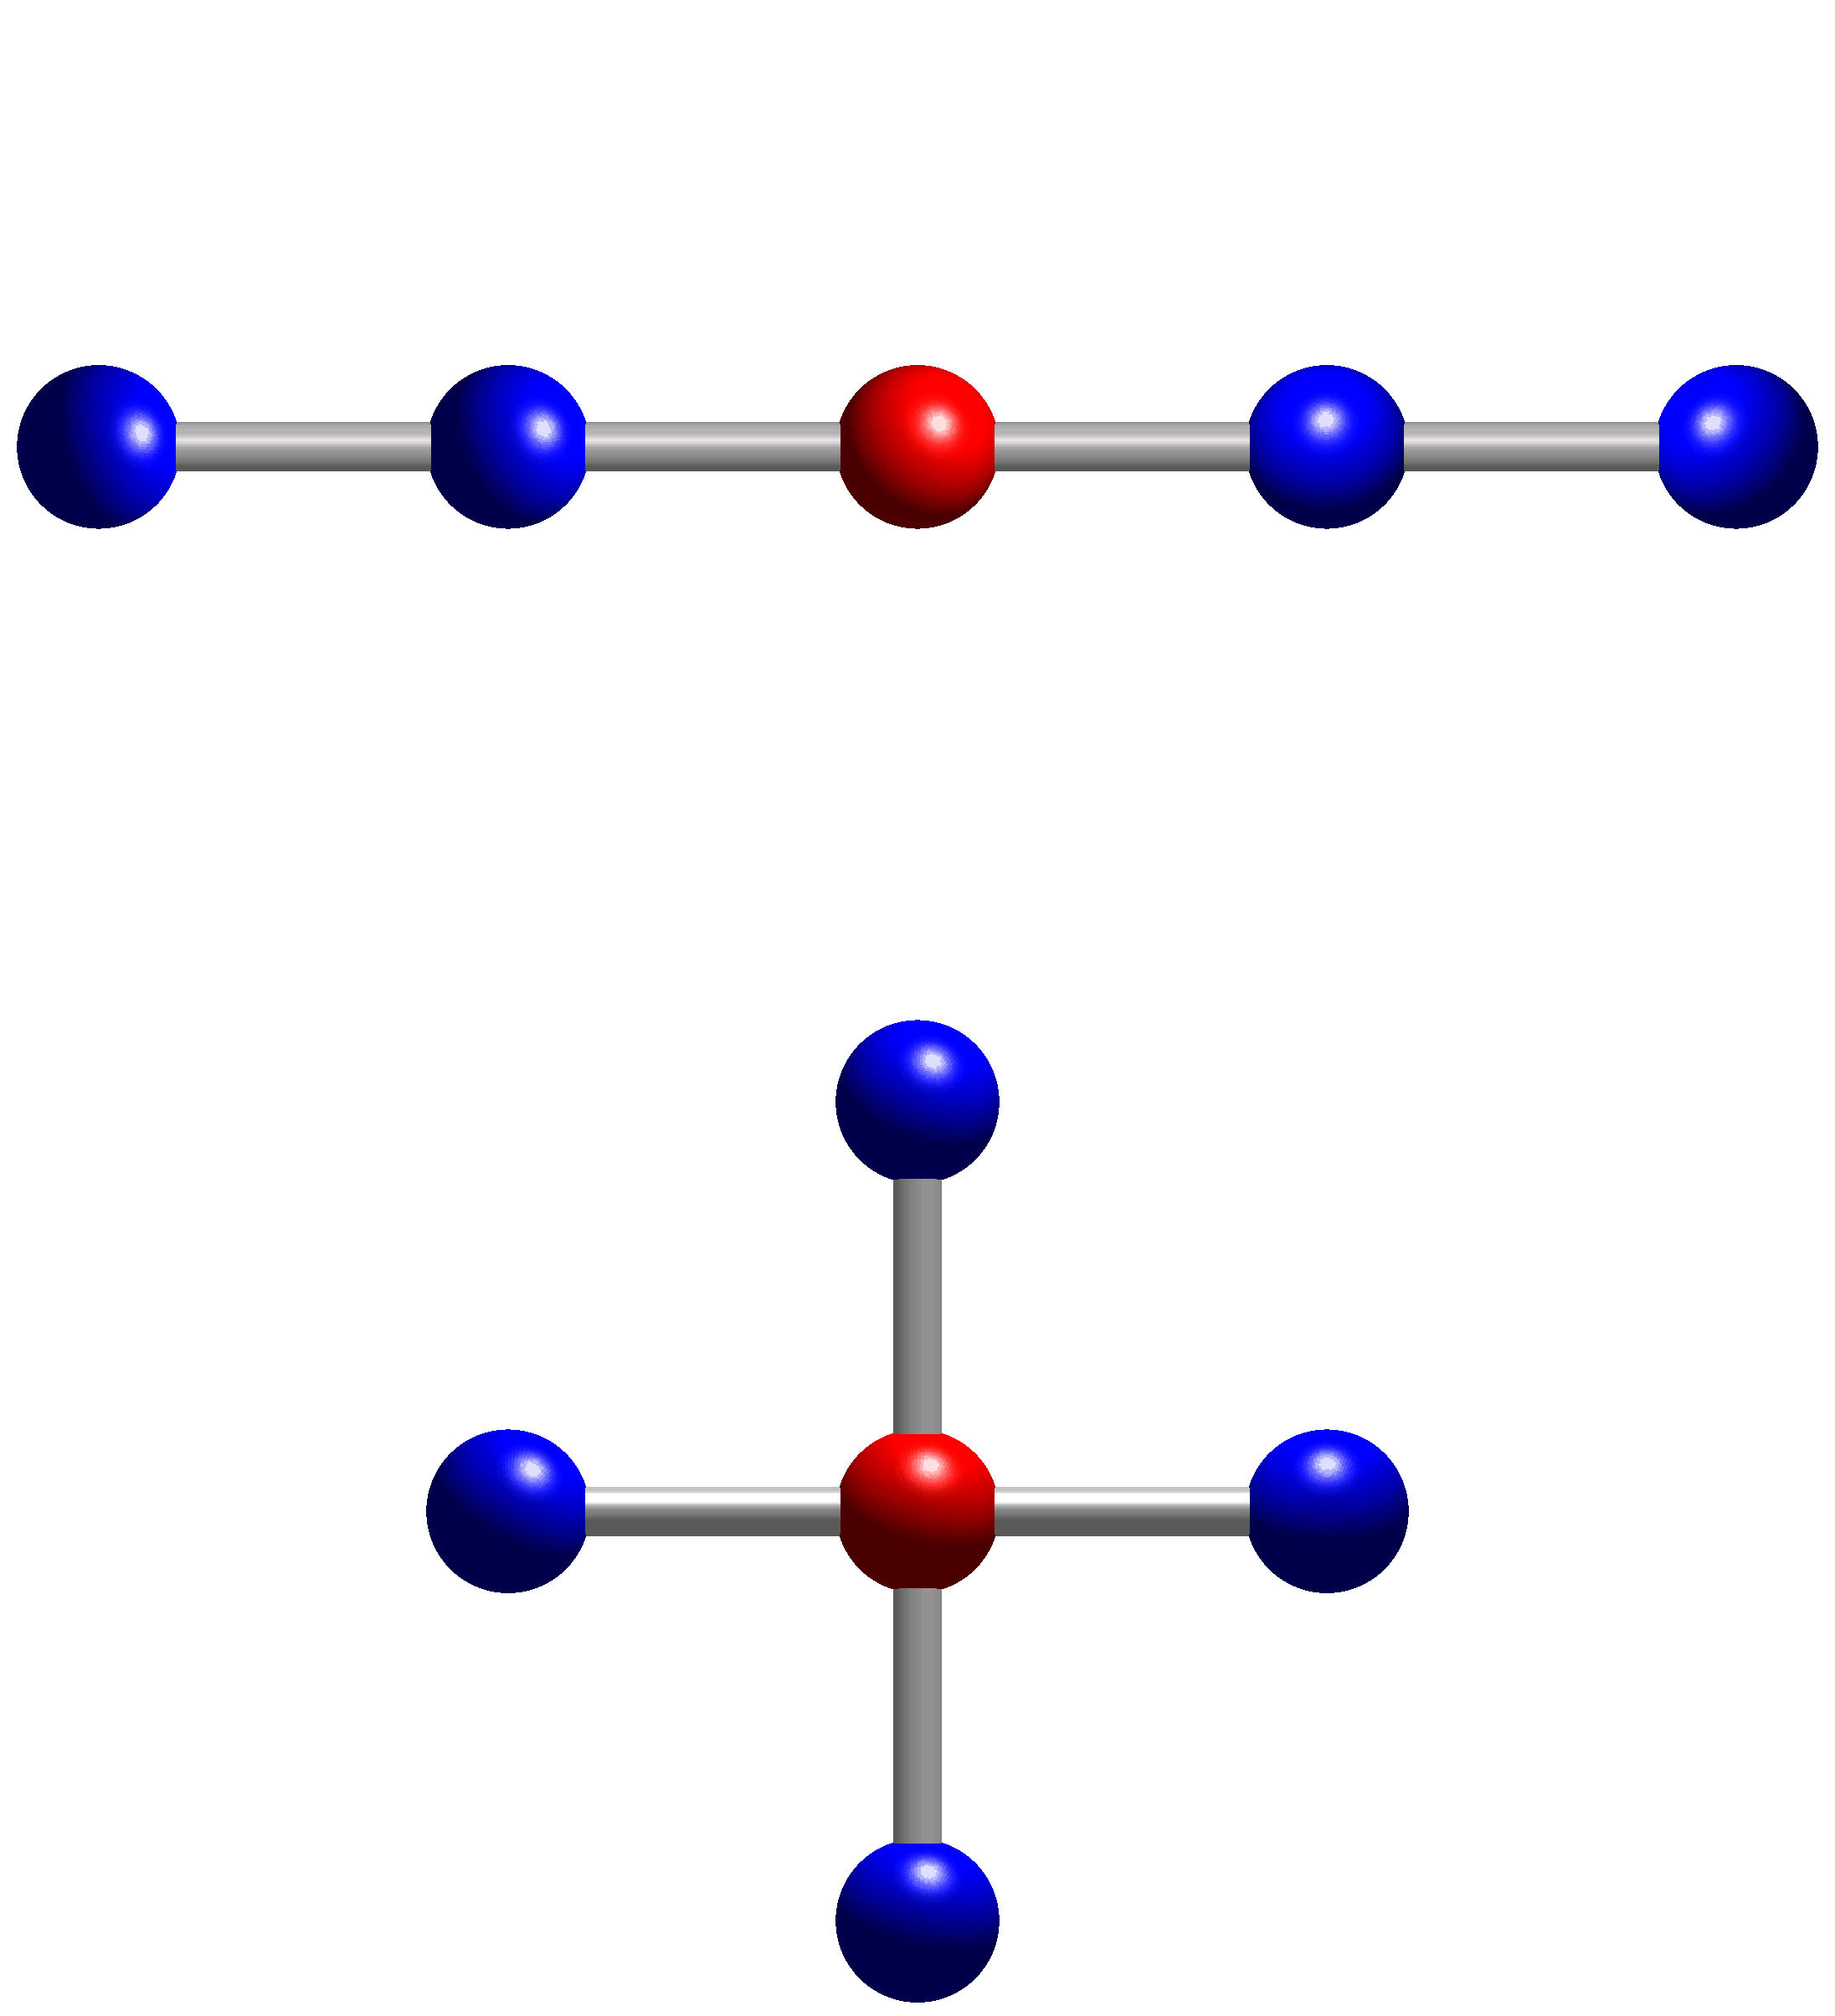
\includegraphics[height=0.5\textwidth]{bilder/I_Five_point_stencil_illustration}
     \caption{1 and 2 dimensional overview of two different 5-point stencils. Illustration taken form \cite{pic1}
     \label{I_Five_point_stencil_illustration.png}}
\end{figure}
A widely used numerical method such as the Finite Difference Method (FDM) are defined to operate over a mesh. I will dive deeper into iterative methods, which are methods used in numerical analysis, in section \ref{subsec:stencil_iteration_types}. 

A mesh is a collection of vertices, edges and faces \footnote{A vertex is a point in the coordinate system, an edge is the connection between two vertices, and a face is a closed set of edges, forming a surface} \cite{article15} that form a polygon mesh. A mesh can be classified as either \textit{structured} or \textit{unstructured}. A structured mesh is identified by a regular connectivity in the mesh pattern. A mesh pattern refers to the geometric alignment of the individual cells in the mesh. Possible element choices for a structured mesh are quadrilateral in 2D or hexahedra in 3D. Structured meshes are easier to evaluate, allow for easy parallelization, and generally require no spatial data structure to manage \cite{article2}. Unstructured meshes are identified by irregular connectivity in the mesh pattern, and can usually be seen as triangles in 2D and tetrahedra in 3D. Unstructured meshes offer the advantage of easier discretization of complex geometries. However they are harder to evaluate, often requiring additional overhead in the form of some spatial data structure, and are generally more difficult to parallelize \cite{article2}, due to its irregular connectivity in the mesh pattern. 
\begin{figure}[!h]
  \begin{center}
    \label{I_structured_mesh.png}
    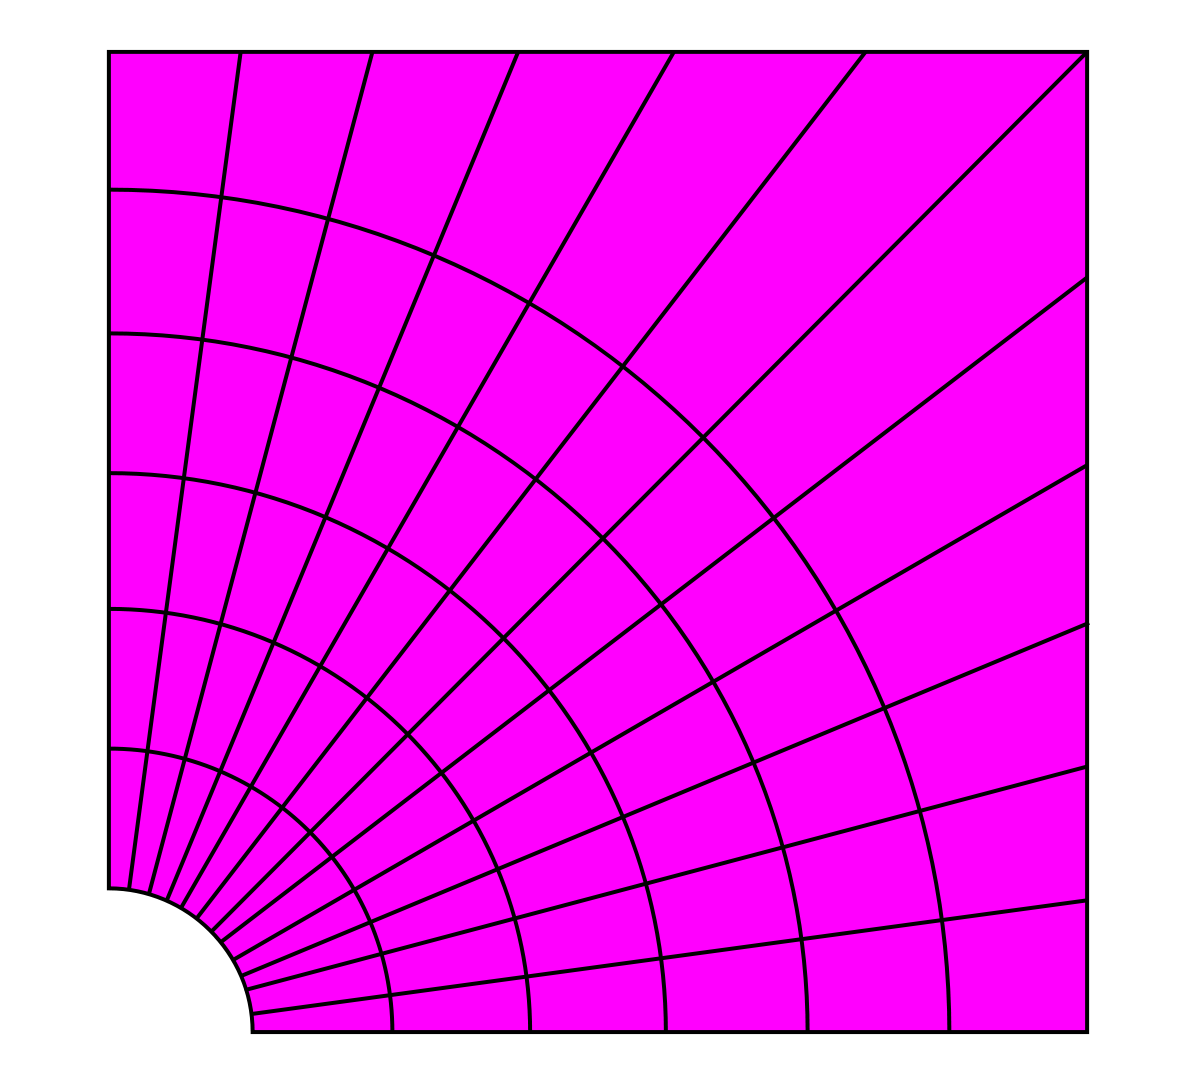
\includegraphics[width=0.45\textwidth]{bilder/I_structured_mesh}
    \label{I_unstructured_mesh.png}
    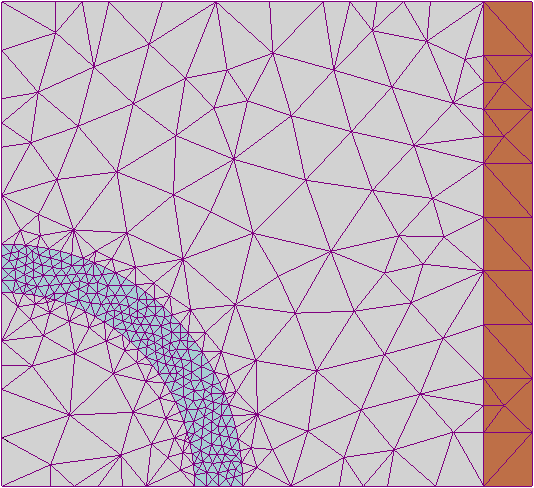
\includegraphics[width=0.45\textwidth]{bilder/I_unstructured_mesh}
  \end{center}
  \caption{Illustration of a structured and unstructured mesh, respectively. Taken from \cite{pic2} and \cite{pic3}}
  \label{I_mesh_types}
\end{figure}

Computations over structured meshes incur regular memory accesses that are easier to achieve, among other things, good cache performance. In comparison, unstructured meshes will include irregular and indirect memory accesses, which are challenging with respect to cache utilization.
A contiguous underlying data storage means that data elements are laid out end-to-end in the memory, with no discontinuities and padding between them, resulting in good memory patterns and high memory efficiency. A few techniques for assuring contiguous memory data storage involves dynamic memory allocation, and loop interchange. Optimization techniques will be discussed in greater detail in section \ref{sec:optimization}. 


\section{Multicore Architectures}
\label{sec:multicore_architectures}
Multicore technology is the most important factor that drives today’s microprocessor performance improvements \cite{article6}. The industry has moved away form exponential scaling of clock frequency toward chip multiprocessors (CMP). A modern computer typically consists of several independent CPU cores on the same socket, each having its own cache, and usually a global memory.  

In computer hardware, there are mainly two different types of memory architecture, \textit{shared}, \textit{distributed}, and a hybrid of these two called \textit{distributed shared} memory. Although the memory architectures mentioned above are old concepts and not only bound to multicore architectures, knowing how the processes in a multicore architecture communicates and store data is essential high performance computing. Shared memory refers to a global address space that can be accessed by several different CPUs. Shared memory is easier to program because it offers an unified address space, although, synchronization is needed, and race conditions among the processes can occur. Shared memory architecture can be of two types, \textit{uniform memory access} (UMA) or \textit{non-uniform memory access} (NUMA). A UMA is when all the processors share the physical memory uniformly \cite{article8} meaning that memory access time is uniformly distributed among the CPU cores. A NUMA architecture means that a processor can access its local memory much faster than the non-local memory since each processor has its own system bus for sending and receiving data from memory. A distributed memory system refers to a system in which each processor has its own private memory region, and interaction between different processes happens over an interconnection network. It excludes race conditions and forces the programmer to think about data distribution in the sense that memory is scalable with the number of processing elements, also referred to as \textit{scalability}. every core should access its local memory unit as much as possible to ensure low latency, and a high memory bandwidth. 

\begin{figure}[!h]
  \begin{center}
    \label{b_distributed_memory.png}
    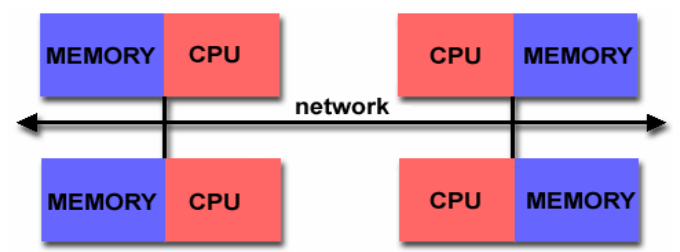
\includegraphics[width=0.45\textwidth]{bilder/b_distributed_memory}
    \label{b_shared_memory.png}
    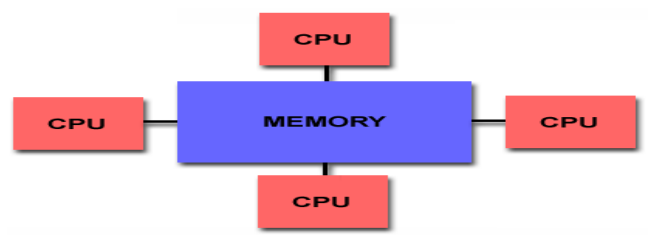
\includegraphics[width=0.45\textwidth]{bilder/b_shared_memory}
  \end{center}
  \caption{overview of distributed and shared memory architecture, respectively. Taken from \cite{article8}}
  \label{b_memory_hierarchy}
\end{figure}

\section{Parallel programming}
\label{sec:problem_decomposition}
\begin{figure}[h]
 \centering 
     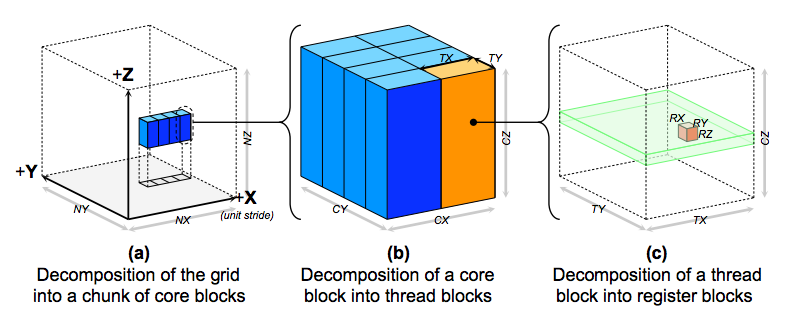
\includegraphics[width=0.9\textwidth]{bilder/b_decomposition}
     \caption{Explaining the decomposition process in a 3 dimensional structured mesh. Illustration taken from \cite{article9}.
     \label{b_decomposition.png}}
\end{figure}
Parallel programming can be split into two categories, shared-memory programming such as Open Multi-Processing (OpenMP), and distributed-memory programming such as the Message Passing Interface (MPI). As discussed in section \ref{sec:multicore_architectures} both memory models have advantages and disadvantages. While OpenMP exploits the shared resources among threads, MPI relies on passing data from one process to another through an interconnection network, each having its own private memory region. In some cases you may want to utilize both programming models, a such technique is often referred to as hybrid parallel programming. In the following example, inspired by \cite{article9}, a hybrid approach can be effectively used to decomposition the problem.

Problem decomposition is one of the most essential stages in a parallel implementation of a problem. Lets assume that we have a large 3D array representing a mesh. To ensure that each processing element gets an equal share of tasks to be executed, we divide the mesh (the entire problem) also referred to as a node block of size \(NX \times NY \times NZ\) into a chunk of core blocks of size (\textit{chunkSize}) \(CX \times CY \times CZ\). By doing so, each process can share its core of blocks. The core blocks are then divided into a series of thread blocks of size \(TX \times TY \times TZ\). Each CPU core usually have multiple threads, decompositioning the problem into thread blocks allows threads to share data which helps reduce capacity misses in the core’s shared cache \cite{article9}. When \( CX = TX\) and \( CY = TY\) there is only one thread per core block. In the third decomposition step, each thread block is then partitioned into register blocks of size \(RX \times RY \times RZ\). Register block optimization involves loop unrolling and jamming, both techniques involves transforming the inner loop. loop unrolling eliminates/reduces data dependency and improves pipelining, while loop jamming reduces loop overhead and gives a better chance for instruction overlap\cite{article10}. The dual of loop jamming is loop splitting. Loop splitting aims to reduce register pressure and remove data dependencies. loop splitting and loop unrolling tends to work really well together if your code has a high number of arithmethic operations. [INTEL]  See examples of loop unrolling and loop jamming below. 
%%https://software.intel.com/en-us/articles/3d-finite-differences-on-multi-core-processors [INTEL]

\begin{lstlisting}[caption=Loop unrolling]
/*A simple example that assumues SIZE is divisible by 4*/
sum = 0;
for(i = 0; i < SIZE; i++)
	sum += a[i]*b[i];

sum = sum1 = sum2 = sum3 = sum4 = 0;
for(int i = 0; i < SIZE-4; i+=4)
{
	sum1 += a[i]*b[i];
	sum2 += a[i+1]*b[i+1];
	sum3 += a[i+2]*b[i+2];
	sum4 += a[i+3]*b[i+3];
}
sum = sum1 + sum2 + sum3 + sum4;
\end{lstlisting}

\begin{lstlisting}[caption=Loop jamming and loop splitting]
/*The innermost loop has been jammed/fussioned to reduce overhead*/
sum = 0;
for(i = 0; i < SIZE; i++)
	for(j = 0; j < SIZE; j++)
		a[i][j] = (b[i-1][j] - b[i+1][j]) + (b[i][i-1j] - b[i][j+1]);

/*The innermost for loop has been split to reduce register pressure*/
for(i = 0; i < SIZE; i++)
{
	for(j = 0; j < SIZE; j++)
		a[i][j] = (b[i-1][j] - b[i+1][j]);
	
	for(j = 0; j < SIZE; j++)
		a[i][j] += (b[i][i-1j] - b[i][j+1]);
}
\end{lstlisting}
%%explain these, then explain unstructured mesh and why its different
%%To ensure that each processing element gets and equal share of tasks to be executed. 
%%TBD: fine-grained parallelism means that you have a large set of small tasks, which tends to be the case in stencil computation as the mesh size can be complex involving many operations.

%%\subsection{Data Allocation} 

\section{Optimization}
\label{sec:optimization}
Stencil optimization can be divided into two categories, stencil-specific, also referred to as source-level optimization, and compiler based optimizations such as auto-tuning. Following the source-level optimization described in \cite{article9}, we can roughly divide these optimizations into three categories.  Data allocation, bandwidth optimization and kernel optimization. 

\subsection{Bandwidth Optimization}
Improving memory bandwidth is a key factor for optimizing stencil computations. Research paper \cite{article9} introduces two methods for effectively increasing bandwidth. \textit{Software prefetching} aims to hide memory latency by allowing data to be moved into the cache before the data are used, and thereby increase effective memory bandwidth. Another way of increasing memory bandwidth is to reduce memory traffic by using a technique called \textit{cache bypassing}. A cache miss is a failed attempt at read or write a piece of data (also referred to as a cache line) in the cache, which requires access to main memory with much higher latency to get that piece of data, causing a great delay in the overall computation speed. As discussed in section \ref{subsec:stencil_iteration_types}, for a Jacobi iteration performing an out-of-place sweep we are only concerned with the write value being written back to DRAM, since the read data is left unused. As showed in \cite{article9}, getting rid of the extraneous reads for a Jacobi iteration using two meshes, you can eliminate \(\frac{1}{3}\) of the overall memory traffic by removing those cache line allocations, resulting in a 50\% improvement in arithmetic intensity, and if you are bandwidth bound, an increase in performance by up to 50\% \cite{article9}.

\subsection{Loop Optimization}
Achieving good temporal and spatial locality is a main concern in stencil computation. Temporal locality refers to the reuse of data, if a memory location is referenced, it is most likely to be referenced again in the near future, thus storing and reusing a copy of the referenced data in a low latency, high memory bandwidth like the cache, yields better performance. Spatial locality refers to the use of neighboring data items. If a memory location is referenced, it is most likely that nearby memory locations will be referenced in the near future \cite{article14}.

as discussed in section \ref{sec:problem_decomposition}, and implemented in \cite{article1}, register blocking involves loop transformations like unroll and jam. There are numerous other ways of optimizing a loop. Following the examples given in \cite{article10} we have \textit{loop interchange}, which involves exchanging the inner loop with the outer loop. This may improve the spatial and temporal locality. Reducing nested loops into a single-nested loop, also known as \textit{loop collapsing} may reduce loop overhead and improve run-time performance \cite{article11}. Another loop transformation technique named \textit{loop peeling} involves performing a problematic iteration separate before entering the loop, with the aim at eliminating dependencies or simplifying a loop. Finally there is cache blocking, also known as loop blocking. Cache blocking  aims to exploit temporal and spatial locality. As illustrated in listing \ref{lst:cacheb} cache blocking is implemented by iterating in sub-blocks of size \(bx \times by\) instead of \(n \times n\). The goal of cache blocking is to find a optimal blocking size small enough to minimize last level cache misses, and large enough to reuse elements already residing in the cache. For the interested reader, other loop optimizations can be found in \cite{article12}.
%%blocking paper after residing in cache

\begin{lstlisting}[caption={Cache Blocking} ,label={lst:cacheb}]
/*Simple example of cache blocking*/
int bx = 64 // block size
int by = 32 // block size
for(ii = 1; ii < n; ii+=by)
 	for(jj = 1; jj < n; jj+=bx)
     	for(i = ii; i <= min(ii+by, n); i++)
         	for(j = jj; j <= min(jj+bx, n); j++)
         		a[i][j] += b[i][j]*c[i][j]*d[i][j]
\end{lstlisting}

\subsection{Auto-tuning}
Now that we have explored a variety of stencil specific optimizations, it is time to move on to compiler based optimization such as auto-tuning. Auto-tuners evaluates a large optimization space by generating variants of a given kernel, as discussed in section \ref{sec:optimization}, and benchmarking its performance. The search effectively tries all the optimizations and reports both peak performance and the most optimal parameters. Auto-tuning is not a new concept and existing libraries include ATLAS and FLAME for dense linear algebra, which involves dot product and matrix multiplication. The sparse linear algebra library OSKI, which involves sparse matrix-vector multiplication (SpMV), and Spiral for spectral methods. The auto-tuning environment created in \cite{article1} encompasses most of the stencil optimizations described in this essay, notably, their optimized stencil is 1.5\(\times\)-5.6\(\times\) faster than the naive parallel implementation, and with a median speedup of 4.1\(\times\)  on cache based architectures \cite{article1}.

%%A modern way of auto-tuning code is by letting the compiler.... SKRIVE MEIR

\subsection{Performance Modelling}
It is important to study the performance of a program with a view of determining the best implementation of a given algorithm. Evaluating the hardware platform, as well as exploiting the benefits of parallelism is essential for achieving high performance. In this section I will introduce essential metrics for analysing the performance of program code.

\subsubsection{FLOPS}
\label{subsubsec:flops}
A commonly used metric for processor performance is given by FLOPS; floating point operations per second. Which is usefull for measuring the floating point operation exectuion rate of a given implementation or computer hardware

\begin{lstlisting} [caption={Loop}, label={lst:forloop}]

 for(j = 1; j < nx; j++)
 	a[i] = (a[i]+ b[i] + c[i])*d[i]

\end{lstlisting}

From example \ref{flops} we can see that the equation in the for loop consists of  2 additions and 1 multiplication, which results in a total of 3 arithmetic operations. From this we develop a simple for calculating FLOPS, which is given in equation \ref{eq1}
\begin{equation} \label{eq1}
\frac{\textrm{Number of Arithmetic operations} \times \textrm{Number of iterations}}{\textrm{Time spent}} 
\end{equation}

If we were to solve example X.X with 3 arithmetic operations, for a total of 
 \(nx = 100 000\) iterations, and time measured executing the for loop is  \(time spent = 0.0004 s\), we get a total of
 
 \begin{equation} 
\frac{3 \times 100 000}{0.0004} = 0.75 \textrm{ GFLOP/s}
\end{equation}

\subsubsection{Speedup}
When evaluating a parallel implementation we are often interested in how much faster the parallel code is compared to the sequential code.
The Execution time of a parallel program is the time that elapses from the moment the parallel program starts to the moment the last processing unit finishes. If the sequential time is denoted by \(T_s\), and the parallel time is denoted by \(T_p\). Then the speedup (S) is defined as ratio of the time taken by best sequential algorithm (\(T_s\)) to the time taken by solving the same problem on \(p\) processing units (\(T_p\)). The equation for calculating the speedup is thus, 

\begin{equation} \label{speedup}
S = \frac{T_s}{T_p} 
\end{equation}

\subsubsection{Bandwidth}
As in the case of determining the computational performance of an implementation given in section \ref{subsubsec:flops}. Another useful metric for determining the memory bandwidth performance of an implementation is to measure the movement of bytes from the memory, to the CPU per second. The memory bandwidth can be attained by calculating the ratio of number of loads multiplied by the datatype (in bytes) and arrays size to the time measured time executing the loop.

\begin{equation} \label{bw}
\frac{\textrm{Number of loads} \times \textrm{Datatype}  \times \textrm{Array size}}{\textrm{Time spent}} 
\end{equation}

Following the example \ref{lst:forloop}, we have a total of 4 loads. Lets assume the elements in the array are of double precision, the number of elements in  each array is 1000, and the time spent executing the for loop is 0.0004 seconds. We get that the memory bandwidth of the implementation is, 

\begin{equation} \label{bwsolved}
Bandwidth = \frac{4 \times 8 \times 1000}{0.0004} =  80 \textrm {MB/s}
\end{equation}

When comparing different implementations, or evaluating different hardware platforms, we are often interested in finding the sustained percentage of the attainable computational rate and memory bandwidth. Which means that you typically use a benchmark library like [STREAM], to find the maximum attainable rate, and compare it to your own measurements.


\section{Stencil Computation Overview}
Stencil calculations perform sweeps through data structures that are typically much larger than the available size of the cache. In addition, data reuse is limited to the number of points in the stencil. As a result, many stencil calculations tends to rely on the speed in which data is transferred from memory to the processor. Therefore, effectively use of the hierarchical memory system such as the different levels of cache, proves to be a key factor in stencil computation performance. Reducing communication overhead that occurs while sweeping through the mesh is also essential for high performance, and parallel programming in general.

\subsection{Stencil Iteration Types}
\label{subsec:stencil_iteration_types}
Partial differential equations (PDE) are very important in science and engineering applications. Iterative Methods for solving PDEs has been extensively studied, and in this section I will cover three stencil iteration types, such as Jacobi, Gauss-Seidel, and Gauss-Seidel Red-Black iterations.

\subsubsection{Jacobi}
Iterative methods such as a Jacobi iteration performs a sweep over a mesh, applying a stencil (nearest-neighbor) to each point in the mesh, called the read mesh. Then the result is written to the corresponding point in the second mesh called the write mesh. The Jacobi method performs out-of-place operations, meaning that both read and write operations requires a distinct mesh. A parallel implementation of Jacobi can be done in an embarrassingly parallel fashion \footnote{A straight forward way of parallelizing a problem}, due to any point in the write mesh can be computed independently of each other. A drawback of Jacobi is that it requires to store distinct read and write arrays, resulting in increased memory storage, and the need for more bandwidth.

\subsubsection{Gauss-Seidel}
Gauss-Seidel iterations performs in-place sweeps, meaning that reading and writing to points are done over the same mesh. There can be several read-only meshes, although, a write mesh must be read from first. A drawback from this is that it limits the amount of available parallelism in the sweep, due to almost all the computed stencils will include some points that were already updated during the current sweep, and others that were not. This means that there is an inherent dependency chain that needs to be respected if we wish to replicate the same final answer \cite{article9}. One benefit from using Gauss-Seidel over Jacobi is that both read and write operations are done using the same mesh, thereby reducing the need for additional arrays, creating less memory traffic and storage requirements. 

\subsubsection{Gauss-Seidel Red-Black}
The Gauss-Seidel Red-Black (GSRB) iteration is similar to Gauss-Seidel in the sense that it performs in-place sweeps. To deal with the limited parallelism that the Gauss-Seidel iteration suffers from, a coloring of points are introduced. A black mesh point will only be updated if all the neighboring red points that it depends on have been updated. This process will continue for all the black mesh points. As a consequence, a GSRB iteration only updates every other point. Making this type of sweep similar in parallelism to Jacobi, since every single-color point can be updated independently of each other.

%%\subsection{Optimization on Unstructured Meshes}
%%\label{subsec:optimization_on_unstructured_meshes}
%%While most research has been devoted to stencil computation over structured meshes, the need for more accurately discretizing complex geometries has led to a rise in the use of unstructured mesh techniques \cite{article2}, \cite{article13}. Most stencil optimization techniques in a regular application consist of exploiting the regular geometric memory access pattern to achieve high performance and maximize the parallelism. Numerical operations over an unstructured mesh tends to yield lower performance and parallelism, due to the different geometric patterns based on the centered point in the stencil. Proved in research paper \cite{article4}, the key to high performance for unstructured tetrahedral meshes lies in a reordering of the tetrahedra, such that the resulting connectivity matrix resembles a block diagonal form where the optimal size of the blocks depends on the hardware \cite{article4}, meaning that carefully fitting the blocks of data in the cache is essential for high performance.

%%Research paper \cite{article2} presents two strategies for evaluating stencil computation over a 2D unstructured triangular mesh, \textit{per-point} and \textit{per-element}. The per-point method iterates over a mesh, and for each point finds all of the triangles that intersect with the stencil centered around that point. The per-element method iterates over a mesh, and for every triangle finds all of the points whose stencil intersects with that triangle \cite{article2}. These two methods tries to maximize data-reuse and data locality. \cite{article2} also claims that the 2D solutions over an unstructured mesh can be extended to 3D unstructured tetrahedral meshes.

%%\section{Related Work}
















